\documentclass[a4paper,10pt]{article}
\usepackage{amsmath}
\usepackage{url}
\usepackage[shadow]{todonotes}
\usepackage{soul}
\usepackage{hyperref}
\usepackage[font=small,format=plain,labelfont=bf,up,textfont=it,up]{caption}
\usepackage{array}
\usepackage[english]{babel}
\usepackage{graphicx}
\usepackage{subcaption}

\DeclareMathOperator*{\argmax}{arg\,max}
\DeclareMathOperator*{\argmin}{arg\,min}
\newcommand{\JanTodo}{\todo[fancyline, color=magenta]}

%opening

\begin{document}

\begin{titlepage}

\newcommand{\HRule}{\rule{\linewidth}{0.5mm}} % Defines a new command for the horizontal lines, change thickness here
\center % Center everything on the page
 
%-------------------------------------------------------------------------------
%	HEADING SECTIONS
%-------------------------------------------------------------------------------

\textsc{\LARGE University of Amsterdam}\\[1.0cm] % Name of your university/college
\textsc{\Large Artificial Intelligence}\\[0.5cm] % Major heading such as course name
\textsc{\large Master Thesis}\\[0.5cm] % Minor heading such as course title

%-------------------------------------------------------------------------------
%	TITLE SECTION
%-------------------------------------------------------------------------------

\HRule \\[0.4cm]
% Title of your document
{ \huge \bfseries Naive Bayes Nearest-Neighbor Object Detection}\\[0.1cm]
{ \large Using Local NBNN and Exemplar-based Models to Solve Computer Vision Tasks\JanTodo{Erg globaal}}\\[0.2cm]
\HRule \\[1.5cm]
 
%-------------------------------------------------------------------------------
%	AUTHOR SECTION
%-------------------------------------------------------------------------------

\begin{minipage}{0.4\textwidth}
\begin{flushleft} \large
\emph{Author:}\\
% Maarten \textsc{van der Velden} % Your name
Maarten van der Velden\\
Student ID: 5743087\\
maarten.vandervelden@\\student.uva.nl
\end{flushleft}
\end{minipage}
~
\begin{minipage}{0.4\textwidth}
\begin{flushright} \large
\emph{Supervisor:} \\
% dr. Jan \textsc{van Gemert} % Supervisor's Name
dr. Jan van Gemert\\
j.c.vangemert@uva.nl
\end{flushright}
\end{minipage}\\[2cm]

% If you don't want a supervisor, uncomment the two lines below and remove the section above
%\Large \emph{Author:}\\
%John \textsc{Smith}\\[3cm] % Your name

%-------------------------------------------------------------------------------
%	DATE SECTION
%-------------------------------------------------------------------------------

{\large \today}\\[3cm] % Date, change the \today to a set date if you want to be precise

%-------------------------------------------------------------------------------
%	LOGO SECTION
%-------------------------------------------------------------------------------


\includegraphics[width=30mm]{Logo}\\[1cm] % Include a department/university logo - this will require the graphicx package
 
%-------------------------------------------------------------------------------

\vfill % Fill the rest of the page with whitespace

\end{titlepage}

\begin{abstract}
    bla
\end{abstract}

% \tableofcontents

% \pagenumbering{arabic}

\section{Introduction} % (fold)
\label{cha:introduction}

\todo[inline]{At the end, review the introduction to see whether the emphasis is correct: should be on the benefits of NBNN, and exemplar model detection..}

Finding objects in images is a main topic in the research area of computer vision. Most methods for finding objects are designed specifically for certain subtopics, such as retrieving one type of objects only, categorizing the scene of the image, or discerning foreground objects from the background. For each of these subtopics, the object finding task is modeled in a certain way. Three very common models are image classification, image segmentation, and object detection.

In image classification (Figure~\ref{fig:classification}), the object finding task is represented as the task of predicting the class of a whole image. The prediction is some measure of how likely it is for an image to belong to a certain class. This task is useful when the image as a whole is of importance, for example when a user is looking for images of a certain topic.

Image segmentation is different from image classification, because for each pixel in the image, a class label has to be found.(Figure~\ref{fig:segmentation}) This task is more complex than classification, because there is less information available for a small patch of the image than for the image as a whole. Therefore, the context of each segment becomes more important for a good classification of objects. Image segmentation might be useful when trying to find the distinction between foreground and background, for example.

Object detection (Figure~\ref{fig:detection}) is similar to both image classification and segmentation, and lies somewhere in between these tasks. Detection is the task of pinpointing areas on an image where objects are, and of which class this object is. Detection is more specific than classification, because the objective is not only to give a class label, but also an indication of the object's location. This indication is not as specific however as in the segmentation task, because the goal is not to define a class for all pixels in the images, but only for the foreground objects. the indication of the object's location can be given in a number of ways, but the most common one is to give a rectangular bounding box that envelops the object \cite{pascal-voc-2007}. Object detection is useful when you are interested in only specific parts of the image, for example in tasks like face detection.

\begin{figure}[hbt]
    \centering
    \begin{subfigure}[b]{0.3\textwidth}
        \centering
        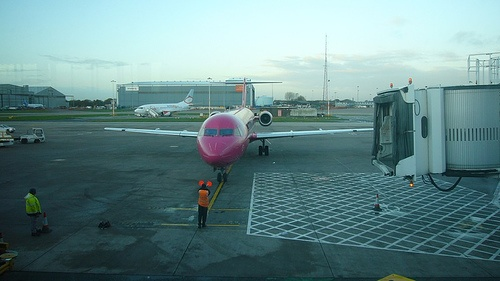
\includegraphics[width=\textwidth]{000032}
        \caption{Classification}
        \label{fig:classification}
    \end{subfigure}%
    ~ %add desired spacing between images, e. g. ~, \quad, \qquad etc.
      %(or a blank line to force the subfigure onto a new line)
    \begin{subfigure}[b]{0.3\textwidth}
            \centering
            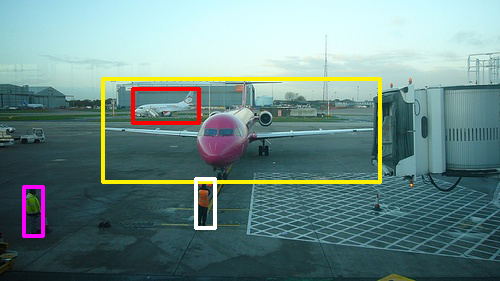
\includegraphics[width=\textwidth]{000032-det}
            \caption{Detection}
            \label{fig:detection}
    \end{subfigure}
    ~ %add desired spacing between images, e. g. ~, \quad, \qquad etc.
      %(or a blank line to force the subfigure onto a new line)
    \begin{subfigure}[b]{0.3\textwidth}
            \centering
            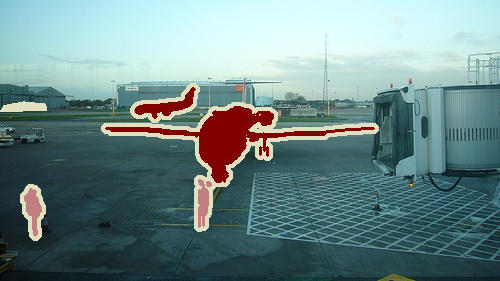
\includegraphics[width=\textwidth]{000032-clsseg}
            \caption{Class-segmentation}
            \label{fig:segmentation}
            \end{subfigure}
    \caption{Three Computer Vision tasks for the same image. If the question is to find persons and airplanes, in a classification task \textbf{(a)} it would be enough to classify the image as a whole as containing both classes. In a detection task \textbf{(b)} bounding boxes need to be given that neatly envelop the objects and have the correct class label. In a class-segmentation task \textbf{(c)}, every pixel should be labeled correctly ``airplane'', ``person'' or ``background'' (transparent in this case). Note that this segmentation image has a blank label for areas that are either on the boundary between different classes, or difficult to classify (at the left side of the image). \cite{pascal-voc-2007}}
    \label{fig:clsdetseg}
\end{figure}

These kinds of algorithms can be used in a broad range of applications. Image retrieval from the internet can be improved by using high level visual data next to textual data such as the filename or context of an image in a web page, especially as the amount of images on the internet grows much faster than they can be for example tagged by useful keywords. Various dedicated systems might use object recognition. For example, in robotics object detection might be used to determine where in the range of the robot certain objects are (and to interact with them accordingly). Another application field is object tracking in video footage. If objects can be successfully detected in single images, it is possible to use this information in an image sequence to learn the trajectories of objects within the sequence. This is useful in surveillance settings, or to gather individual statistics of players in team sports. \cite{benfold2011stable, ekin2003automatic, lipton1998moving}

For image classification, recently the Naive Bayes Nearest Neighbor (NBNN) \cite{boiman2008defense} approach has gained popularity. \cite{becker2012codebook, behmo2010towards, mccann2012local, timofte2012iterative, tuytelaars2011nbnn, wang2011improved, zhang2010random} Boiman \emph{et al.} apply the simple nature of nearest-neighbor classification to build a state-of-the-art image classification method. They show that a Nearest-Neighbor based approach for image classification has a number of appealing properties. In the first place, Nearest Neighbor is a so-called ``lazy'' classification method, meaning that it does not need a separate phase in which it learns a model. It does not build a model for a decision boundary based on the evidence given, but is just compares each query directly with this evidence. This also makes the method parameter-free, meaning that there are no parameters needed that influence the model that is made.

Because no model is learned, the raw evidence is of much importance in NBNN, therefore the more evidence is available, the better. Parametrized methods benefit from little but good evidence, but without a learning step, the quantization error this gives is very harmful. Furthermore, Boiman shows that query images should not be compared to evidence images, but to the aggregated evidence classes, image-to-class distance.

Among improvements by others, McCann \& Lowe \cite{mccann2012local} have come up with an adaptation of NBNN which looks at the local surroundings of image features in the NN-space across all classes in stead of a class-by-class approach. This Local NBNN (LNBNN) approach uses more than one single nearest neighbor to find object-to-class distances to multiple classes at once, making the process more efficient and the performance better. 

In this thesis I will explore the possibilities of extending the NBNN method from image classification to object detection. I combine McCann \& Lowe's LNBNN based object-to-class distance estimation with exemplar-model object detection \cite{becker2012codebook, chum2007exemplar}. To do this, each object descriptor taken during training is regarded as an exemplar. It refers to a certain part of the object it was sampled from. In this way, bounding box hypotheses can be made from descriptors in a test image and their nearest neighbor exemplars. These hypotheses can be clustered to form detections. In this regard, single-link agglomerative clustering as used by Becker \emph{et al.} \cite{becker2012codebook} is compared with quickshift mode finding clustering .

The tests are performed on both a composed dataset of motorbike images \cite{becker2012codebook, fritz2005integrating}, and on the challenging VOC2007 object detection task \cite{pascal-voc-2007}.

\todo[inline]{Make sure all experiments are mentioned and shortly explained in here, and it is made clear what the benefit of the method is, before the next (last) section.}

Section~\ref{cha:related_work} gives an overview of related work on the various parts of this task. In Section~\ref{cha:naive_bayes_nearest_neighbor} I will discuss the details of the NBNN method, and the assumptions under which it works. In Section~\ref{cha:object_detection} the theory behind exemplar-based modeling will be explained. The link between the two methods will be made in Section~\ref{cha:linking}. In Section~\ref{cha:experimental_setup} the experiments will be elaborated, after which the results are given. In Section~\ref{cha:analysis_of_results} these results are discussed and analyzed. Finally, in Section~\ref{cha:conclusion} conclusions will be drawn and discussed.

% section introduction (end)
\section{Related Work} % (fold)
\label{cha:related_work}
\todo[inline] {Needs revision and expansion (shorten the obvious parts, expand on interesting NBNN \& detection related papers)}

\subsection{Image Classification} % (fold)
\label{sec:image_classification}
\todo[inline]{Talk of related non-NBNN classification methods}
\JanTodo{BoW, Fishor, Devil in the Details, BMVL, Chatfield}
% section image_classification (end)

\subsection{Image Detection} % (fold)
\label{sec:image_detection}

\todo[inline]{Talk of related non-NBNN detection methods (Get part based models and the like in here \ldots )}

\todo[inline,color=green]{Next part comes from the Detection chapter, revision needed, and include something on exemplar models}

The most intuitive way of thinking about object detection is probably to apply image classification at various windows within the image instead of on the image as a whole. This involves iterating over possible window locations, sizes and aspect ratios for the whole image, and determining the likelihood of each window of representing an object. This so called sliding window approach marks early detection methods \cite{viola2004robust}. The applicability of this approach however is fairly limited, because of the large number of possible windows to check. Therefore, many methods find a way to make this window search more efficient. Viola \& Jones \cite{viola2004robust} propose a cascade approach, where a very simple classification method is used on the full set of hypotheses for bounding boxes in order to cast most of them away early. For difficult hypotheses a more sophisticated classification is done to narrow down the search, each step using a better, and much slower classification algorithm. In contrast, Efficient Sub-window Search methods \cite{behmo2010towards, lampert2008beyond, pedersoli2011coarse, yeh2009fast} model the problem into a branch-and-bound search method. They recursively split the window in two, find the response for the class on the current scale, and continue with the most promising leaf. When the response of both windows after a split is lower than the one above, the correct window is assumed to be on the above level.

Another approach that recently gained more attention\JanTodo{why?} is that of detection by segmentation.\cite{van2011segmentation,zhang2010free} These methods rely on the fact that segmentation methods are meant to subdivide the image into segments that represent a semantic unity, like parts of objects or full objects. The resulting segments can be used as hypotheses for detecting objects. This means the amount of possible windows can be reduced heavily. Van de Sande \emph{et al.} \cite{van2011segmentation} use a hierarchical segmentation algorithm to make the detection scale invariant, and train discriminatively by focusing on hard examples. Zhang \emph{et al.} \cite{zhang2010free} do not explicitly segment the image, but just like many segmentation algorithms they do look for edges that enclose an object as a restraint for selecting it as a possible detection.

Part-based models form a different approach on effectively finding hypothesis windows for objects \cite{felzenszwalb2010object}. These methods learn object models based on a combination and spatial organization of a number of designated, but unlabeled, parts. These parts are learned as a hidden variable during training, being groups of features reoccurring in the same formation in a certain area of bounding boxes of a class. Furthermore, the difference in scale between the full object window (the root) and its parts is fixed. In comparison with sliding-window approaches, this means a restriction in the number of possibilities for detection of objects. The relative scale of the parts should comply with that of the root scale. \todo{need to cite these, perhaps briefly mention them before...?}

\begin{figure}[hbt]
    \centering
    \missingfigure[figwidth=0.8\textwidth]{Show images of the idea comparing the methods discussed}
\end{figure}

% \todo[inline,color=red]{Next part comes from previous subsection of introduction, To Be Reviewed...}.

% With a choice of image descriptors, a class description and a training method, image classification can be performed. For object localization within an image however, a strategy is needed to estimate classifications for parts of images instead of images as a whole.
% 
% The most straightforward method is to take a window on a test image, and to classify that part of the image as if it were an image in itself. This sliding window approach \todo[fancyline]{reference} is just a small conceptual step, but generates a lot of possible windows to be classified, therefore costing much computation. This hampers the applicability of this naive method. Smarter versions of this approach include include a divide-and-conquer tactic called branch-and-bound search. \cite{lampert2008beyond} In this method, a fitness (response) of the current window is calculated, and then the window is subdivided in two non-overlapping windows, the most promising of which is iteratively subdivided until the globally highest fitness is found. However being much faster than the vanilla sliding window approach, it has the disadvantage of covering hard boundaries between sub-windows, making it hard to find exact locations of objects.
% 
% Part-based models have a different approach. This method models classes with special regional descriptors which define the relative orientation and scale of parts of an object with respect to the location and size of the object as a whole. \cite{leibe2004combined, chum2007exemplar, felzenszwalb2010object} These descriptors enable the detection algorithm to look for the arrangement of descriptors in a test image, and to define the most likely locations of objects. Some methods expand this into trying to create 3D models of classes, to make matching rotation independent. \todo[fancyline]{reference}

% section image_detection (end)

\subsection{NBNN Based Methods} % (fold)
\label{sec:nbnn_based_methods}
\todo[inline]{Talk of Boiman shortly, and of methods related to it, up till the most recent ones, so include Becker, Wang, Behmo, McCann, Tuytelaars, etc.\ldots}
% section nbnn_based_methods (end)

\subsection{Image Descriptors} % (fold)
\label{sub:image_descriptors}

\todo[inline,color=red]{Removed in the future(?)}.
\JanTodo{Needed? Maybe in Introduction: \textbf{Why the problem is hard}}
% To be able to make a description of each object class, a representation of each (part of an) image is needed that best captures the informative aspects of the objects. The most basic descriptor type is to use the pixel values of the image. These capture the image exactly and might therefore seem very useful as descriptors of object types. The problem however with pixel values, is that images tend to vary wildly in them, even though the exact same object might pictured.

% There are a number of types of variation that may be expected when comparing arbitrary images of the same object type:
% \begin{description}
%     \item[Camera] Use of different cameras and compression algorithms (image filetypes) will cause a change of pixel values. Images might be darker or lighter, have a different balance of colors, more or less color depth, etc.
%     \item[Scene] Lighting of the scene may cause significant changes in pixel values, because of the change in intensity or in spectrum. Also, the background behind the object might change
%     \item[Orientation] Transformation of the object with respect to the image frame. An object might be on an arbitrary location in the image, rotated in various angles, viewed from up close or from far away.
%     \item[Occlusion] Objects might be partially out of sight, because they are not framed entirely, or because something is in front of them.
%     \item[Intra-class-variation] Objects from a single class may vary wildly in appearance. Imagine a number of objects that qualify as a chair, and how different these might look.
% \end{description}
% Therefore, raw pixel values might not be a very good choice as description on its own
% \todo[inline]{connect this with other descriptors, be shorter than now, focus on sift as that's what I'll use, give SIFT's advantages and limitations. Meaning TODO: revision of the following}
% 
% In general, there are three kinds of descriptor types: global, regional and local descriptors. Pixel values are a type of local descriptors. These descriptors capture the local information (in this case at pixel level) very well, but they don't take their context into account. This is what regional descriptors do. They describe in a concise way what is to be derived from a small region of pixels in an image. Usually, these describe local changes in intensity, edges, lines, corners or blobs, and are very popular in computer vision. Global features describe characteristics of the image as a whole. 
% 
% Very often, multiple kinds of descriptors are used together to make a description of an image, and of objects.

% subsection image_descriptors (end)

\subsection{Training Methods} % (fold)
\label{sub:training_methods}
\todo[inline,color=red]{Removed in the future(?)}.
\JanTodo{Needed? Maybe in Introduction: \textbf{Why the problem is hard}}


% \todo[inline]{Better be incorporated in the previous subsections, otherwise it will be too much repetition... small piece on BoF and similar methods. small piece on the following subsection. Perhaps at the end of the NBNN section, as `other classification methods'??}
% 
% \todo[inline]{(perhaps diverge a little to other methods that use NN and detection, but in a different way (SVM-kNN, galleguillos, etc.), !related work section!, but I dropped that, lets see later on).}
% 
% 
% With the representation of images, it becomes possible to make a model for each object class to be detected. In this way, test images can be matched with each class model to find out which is the most likely.
% 
% To be able to make a class description, sample images are needed, annotated with a description of what the image represents. This is the training set. From this set, the descriptors found can be labeled with the correct class, so a description of each can be made. Usually this is done in a learning phase.
% 
% 
% Bag of Words is another popular method \cite{lazebnik2006beyond, van2011exploiting} \todo[fancyline]{continue this as an overview}

% subsection training_methods (end)

% chapter related_work (end)
\section{Naive Bayes Nearest Neighbor} % (fold)
\label{cha:naive_bayes_nearest_neighbor}

The focus of this thesis is on the Naive Bayes Nearest Neighbor (NBNN) image classification method, first presented by Boiman \emph{et al.} \cite{boiman2008defense} In this section the theory behind the method, its sources and its later adaptations will be discussed.

\subsection{$k$-Nearest Neighbor Classification} % (fold)
\label{sub:_k_nearest_neighbor}

The $k$-Nearest-Neighbor algorithm is one of the earliest approaches for classification in machine learning. Given a set of items $n \in \mathcal{N}$, labeled with a designated number of classes $c_n \in \mathcal{C}$, an unlabeled query item $q$ and a distance measure to calculate pairwise differences between items $d(x_1\|x_2)$, the nearest neighbors of $q$ are the $k$ items in $\mathcal{N}$ for which $d(q\|n)$ is lowest. In turn, sets $\text{NN}_c(q)$ contain those nearest neighbors of $q$ that belong to class $c$. This way, $k$NN classification comes down to
\begin{align}
    \hat c_q &= \argmax_c |\text{NN}_c(q)|,
\end{align}
being the class of which the most items are within the $k$ nearest neighbors of $q$.

In contrast to other classification algorithms, $k$NN is relatively simple. It does not require any training to make a model from the labeled images. The algorithm only estimates the probability density of the classes locally, within $k$, which means it does not assume a global probability density distribution underneath the data, which makes it a non-parametric way of making a non-linear classifier.

\subsection{Naive Bayes Classification} % (fold)
\label{sub:NB}

Naive Bayes is another rather simple classification algorithm, which is based on the idea that a simplification of Bayes' Theorem can be made using the assumption that all features of an item $d_{n,i} \in \mathcal{D}_n$ appear conditionally independent of each other. This means that $p(d_{n,i} | c_n, d_{n,j}) = p(d_{n,i}|c_n)$ is assumed for all $n,c,i,j, i\neq j$. 

If Bayes' Theorem is modeled to predict the probability of a class $c$ of an item $q$, we can say
\begin{align}
    \label{eq:bayes}
    p(c|q)      &= \frac{p(q|c)\,p(c)}{p(q)}\\
                &\propto p(q|c)\,p(c),
\end{align}
because the probability is to be compared among all classes $\mathcal{C}$, for the same item $q$, which makes $p(q)$ constant. Furthermore, if $q$ is represented by $m$ features $d_q$, \eqref{eq:bayes} can be rewritten as
\begin{equation}
    p(c|d_{q,1},\dotsc,d_{q,m}) = p(d_{q,1}, \dotsc,d_{q,m}|c)\,p(c),
\end{equation}
which is equivalent to the joint probability
\begin{align}\begin{split}
    p(c|d_{q,1},\dotsc,d_{q,m}) &\propto p(c,d_{q,1}, \dotsc,d_{q,m})\\
        &\propto p(c)\,p(d_{q,1}|c)\, p(d_{q,2}|c,d_{q,1}), \dotsc,p(d_{q,m}|c,d_{q,1},d_{q,2},\dotsc,\\&\quad d_{q,m-1}).
    \end{split} 
\end{align}
By the conditional dependence assumption made above, this can be reduced into
\begin{equation}
    p(c|q) \propto p(c)\prod_{i=1}^m p(d_{q,i}|c).
\end{equation}
With this equation, a decision rule can be made as follows
\begin{equation} \label{eq:map}
    \hat c_q = \argmax_c \frac{1}{m}\,p(c)\prod_{i=1}^m p(d_{q,i}|c),
\end{equation}
which is called a maximum a-posteriori (MAP) classifier. In this formulation of a classification problem, a probability density estimation is needed to model all features. All kinds of distributions can be used for this.

\subsection{Boiman's NBNN} % (fold)
\label{sub:boiman_s_nbnn}
Boiman \emph{et al.} \cite{boiman2008defense} coined the term Naive Bayes Nearest Neighbor (NBNN) for their image classification algorithm, that used a combination of Nearest-Neighbor (NN) and Naive Bayes to classify images in a multi-class setting. The approach works well because of the non-parametric character of the approach, which means no parameter learning is required. This makes it easy to use the method on a problem with a large number of classes, while parametric methods typically model multi-class problems as multiple 2-class problems. It also means that the risk of overfitting is smaller because there are no model parameters to be tuned. The only parameters are in the (type and amount of) features, which is the same for other classification methods. The authors achieved results competitive to the state of the art Bag of Features (BoF) methods because the method benefits from two requirements it meets: (\emph{i}) Avoiding feature quantization and (\emph{ii}) the use of image-to-class distance instead of image-to-image distances. They theorize that earlier attempts to use NN \cite{berg2005shape, zhang2006svm} for image classification failed because these do not meet both requirements.

\begin{figure}[hbt]
    \centering
    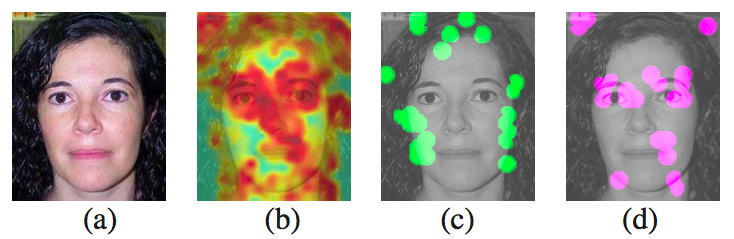
\includegraphics[width=0.8\textwidth]{QuantizationError}
    \caption{Visualization of the quantization error. (a) An image from the Face class in Caltech101. \cite{caltech101} (b) ``Quantization error of densely sampled SIFT descriptors using a large codebook of Caltech101. Red = high error; Blue = low error. The most informative descriptors (eye, nose, etc.) have the highest quantization error.'' (c) ``Green marks the 8\% of the descriptors in the image that are most frequent in the database (simple edges).'' (d) ``Magenta marks the 8\% of the descriptors in the image that are least frequent in the database (mostly facial features)''. From \cite{boiman2008defense}}
    \label{fig:quantization_error}
\end{figure}

Feature quantization is a means of creating compact image descriptions, such as the ones used in the BoF methods. In BoF, all descriptors of an image are clustered into visual words, and histograms are constructed counting the occurrence of each word in an image. Image matching is based on comparing these histograms. Quantization is harmful for a nearest neighbor approach because the most informative descriptors get the highest quantization error while being necessary for finding nearest neighbors. This becomes clear when the observation is made that for a descriptor to be more informative, it should appear only at certain circumstances, ideally only in images of one class. They should be fairly well recognizable among other descriptors, and therefore they tend to be outliers in descriptor space. When quantizing, these descriptors will mostly be incorporated into visual words that are rather unlike these descriptors, resulting in a large quantization error. In Figure~\ref{fig:quantization_error}, the effects of this are illustrated.

In learning-based methods, like SVM, this quantization error is outweighed by the benefit of dimensionality reduction which allows training on a large data set. Furthermore, the problem itself is mitigated in BoF methods. The learning phase in these methods makes sure that only descriptors that are good predictors, regardless of their quantization error, are considered in the test phase. Because NBNN does not have a training phase nor dimensionality reduction, it has to use every single descriptor of each image to perform NN on, to avoid the quantization error.

Kernel methods such as SVM are based on image-to-image distances to create decision boundaries. For each image in the training set, a histogram of visual words is built, based on the features that appear in the image, and are matched with the visual words that resulted from quantizing all training features. 
In a nearest neighbor approach, image-to-image distances do not enable much generalization, as no inference is done from the training images and their features. This would mean only test images close to known images will be classified correctly. Therefore, image-to-class distances should be used. While an image might be far removed from all others of a certain class, the individual features might all be close to features of different images of this class, making the image-to-image distances to a class large, but the image-to-class distance short. \cite{wang2009learning} Figure~\ref{fig:im2im_vs_im2cl} shows the difference between image-to-image distance and image-to-class distance.

\begin{figure}[hbt]
    \centering
    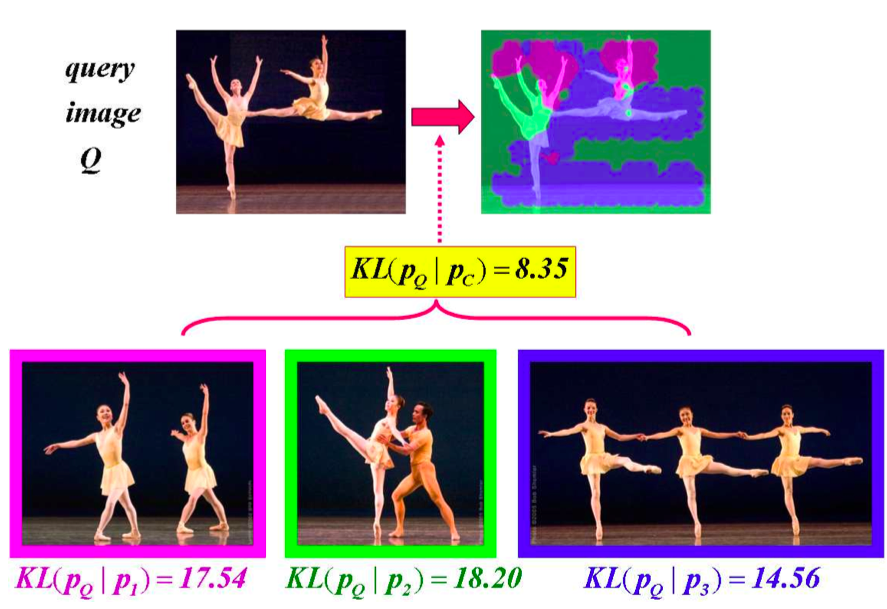
\includegraphics[width=0.8\textwidth]{Im2imVsIm2cl}
    \caption{Image-to-class distance versus image-to-image distance. Given three labeled images of the ``ballet''-class (bottom row), and a query image (top left). Even though the ``Query-to-image'' distance is large to each individual labeled image, represented by the KL-divergences, the ``Query-to-class'' distance is small. The top right image shows the query image, with each descriptor having the color of the labeled image which gave it the highest descriptor likelihood. It shows that this query configuration is more likely given the three images, than each individual image separately. (Image taken from \cite{boiman2008defense, irani2006similarity}.)}
    \label{fig:im2im_vs_im2cl}
\end{figure}

Using the main points of no quantization and image-to-class distances, $k$-nearest neighbor can be performed for individual features, per class. Note that in this way, each individual feature could be classified as its NN, but a second step is required to classify images as a whole. Therefore the set of individual distances is used as the input of a Naive Bayes classifier.

The NBNN decision rule is defined under the Naive Bayes assumption of Section~\ref{sub:NB}. The MAP classifier from \eqref{eq:map}, when assuming uniform priors $p(c)$ over all classes, simplifies to Maximum Likelihood (ML) classifier 
\begin{align}
    \hat c &= \argmax_c \frac{1}{m}\prod_{i=1}^{m} p(d_{q,i}|c)\\
           &\propto \argmax_c \frac{1}{n}\sum_{i=1}^{n} \log p(d_{q,i}|c),
\end{align}
Where the last formulation as a sum of log-probabilities is used in practice to compensate for the low probabilities typical for this classifier, which may cause rounding errors in computer applications.

Using the notion that NN classification tends to the Bayes optimal classifier when the sample size tends to infinity\cite{boiman2008defense, cover1967nearest}, dense sampling can be used to get a high number of descriptors per class from the training set $Z = |\mathcal{D}_c|$. The class conditional probability of a feature $p(d_q|c)$ can be modeled using Parzen likelihood estimation, where
\begin{equation} \label{eq:parzen}
    \hat p(d_q|c) = \frac{1}{Z}\sum_{j=1}^L K(d_q-d_{c,j}).
\end{equation}
Parzen kernel function $K(\cdot)$, typically Gaussian, defines the distance between query descriptor $d_{q}$ and labeled descriptor $d_{c}$. When $Z$ goes to infinity, $\hat p(f|c)$ approaches $p(f|c)$. 

This approach entails calculating the distance of $d$ to all $Z$ descriptors of each class, which would be very costly. Because only a small minority of the descriptors can be expected to be significantly close to $d_q$, taking into account only the nearest descriptors is a safe approximation, which enables using nearest neighbors (NN) to find these descriptors. Even more so, Boiman shows that the performance loss of taking only the 1 nearest neighbor is very small. Because of this the Parzen estimate of $d_q$ to class $c$ reduces to the distance of $d_q$ to its nearest neighbor in $c$: $\|d_q - \text{NN}_c(d_q)\|^2$, resulting in the following log likelihood and classifier: 
\begin{align}
    \label{eq:nbnnloglikelihood}
    \log P(q|c) &\propto -\sum_{i=1}^m \|d_{q,i} - \text{NN}_c(d_{q,i})\|^2 \\
    \label{eq:nbnnclass}
    \hat c      &= \argmin_c \sum_{i=1}^m \|d_{q,i} - \text{NN}_c(d_{q,i})\|^2
\end{align}

Now, classification boils down to calculating descriptors for all images in each class and for the query image, estimating the nearest neighbor of each query descriptor for each class, calculating the sum of distances for each class for the query image and selecting the lowest distance. This approach is both very simple and intuitive. It also enables use of different kinds and combinations of descriptors.

% subsection boiman_s_nbnn (end)


\subsection{Limitations and Extensions} % (fold)
\label{sub:limitations_and_extensions}

Even though the algorithm of Boiman \emph{et al.} \cite{boiman2008defense} is very simple and requires no learning phase, it does have scalability issues because of its dependence on as many individual descriptors as possible. Because all densely computed descriptors for each image in the training set have to be stored, and the nearest neighbor for each descriptor of each query image on each class has to be found, the time and memory usage is much higher than for example BoF methods, which use a more compact representation of images. Calculating NN can be sped up by using sophisticated approximations of the Nearest Neighbor algorithm, such as FLANN \cite{muja2009fast}, which uses randomized kd-trees to provide a quick search in a k-dimensional search space. This relieves some time issue, but is not a remedy for the memory issues.

% section limitations_and_extensions (end)

\subsubsection{Local NBNN} % (fold)
\label{sec:local_nbnn}

An adaptation of NBNN by McCann \& Lowe called local NBNN (LNBNN)\cite{mccann2012local} has another approach to solve some of the limitations of the original algorithm. Their main idea is that it is not necessary to find a descriptor's nearest neighbor in each class, but that is sufficient to find the $k$ nearest neighbors over all classes. It will perform better, in fact. See Figure~\ref{fig:lnbnn} for a visualization of the conceptual difference.

The simplification of the basic query implies a more efficient algorithm, because it is much faster to search for $k$ nearest neighbors in one collection, than to search for 1 NN for each class, even when $k$ is much larger than the number of classes.

Besides the time-complexity benefit, LNBNN also enhances the results of NBNN. Because only the $k$NN are taken into account, it might well be that not all classes will be involved for each descriptor in an image. In the original NBNN, these distances would still be taken into account, lowering the chance of the class to get the highest probability for the image by a possibly large amount. LNBNN takes the $k+1$-th distance for these classes, making this effect much less significant. Liu \emph{et al.}\cite{liu2011defense} have hypothesized that in a sparse manifold space, such as the descriptor space, larger distance give a much worse estimate of membership to a class. This might be the cause for the improved results LNBNN gets compared to Boiman's NBNN. Another argument is that each descriptor should at most add a bit evidence to the probability of an object's class. It should not lower this probability. Otherwise the influence of background clutter could be too large.

LNBNN will be used as a basis for the object detection algorithm, because it is an efficient variant of NBNN, and extends to the $k>1$ case, which proved to be important in the detection case.

\begin{figure}[hbt]
    \centering
    \begin{subfigure}[b]{0.60\textwidth}
        \centering
        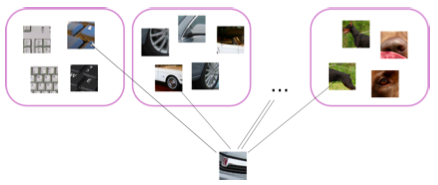
\includegraphics[width=\textwidth]{LNBNNa}
        \caption{The original NBNN asks, ``Does this descriptor look like a keyboard? a car? \ldots a dog''}
        \label{fig:lnbnna}
    \end{subfigure}%
    ~ %add desired spacing between images, e. g. ~, \quad, \qquad etc.
      %(or a blank line to force the subfigure onto a new line)
    \begin{subfigure}[b]{0.30\textwidth}
        \centering
        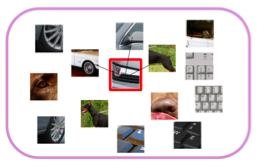
\includegraphics[width=\textwidth]{LNBNNb}
        \caption{Local NBNN asks, ``What does this descriptor look like?''}
        \label{fig:lnbnnb}
    \end{subfigure}%
    \caption{Difference in conceptual approach of regular NBNN and Local NBNN. From \cite{mccann2012local}.}
    \label{fig:lnbnn}
\end{figure}

% subsection local_nbnn (end)


% section naive_bayes_nearest_neighbor (end)
\chapter{Object Detection Using Exemplar Models} % (fold)
\label{sec:object_detection}

\begin{figure}[hbt]
    \centering
    \missingfigure[figwidth=0.8\textwidth]{Show images of the idea comparing the methods discussed}
\end{figure}

The most intuitive way of thinking about object detection is probably to apply image classification at various windows within the image instead of on the image as a whole. This involves iterating over possible window locations, sizes and aspect ratios for the whole image, and determining the likelihood of each window of representing an object. This sliding window approach marks early detection methods.\cite{viola2004robust} The applicability of this approach however is fairly limited, because of the large number of possible windows to check. Therefore, lot of methods find a way to make this window search more efficient. Viola and Jones\cite{viola2004robust} propose a cascade approach, where a very simple classification method is used on the full set of hypotheses for bounding boxes in order to cast most of them away early. On the difficult hypotheses a more sophisticated classification is done to narrow down the search more and more, each step using a better, and much slower classification algorithm. In contrast, Efficient Sub-window Search methods\cite{ lampert2008beyond, yeh2009fast, pedersoli2011coarse, behmo2010towards} model the problem into a branch-and-bound search method. They recursively split the window in two, find the response for the class on the current scale, and continue with the most promising leaf. When the response of both windows after a split is lower than the one above, the correct window is assumed to be on the above level.

Another approach that recently gained more attention is that of detection by segmentation.\cite{van2011segmentation,zhang2010free} These methods rely on the fact that segmentation methods are meant to subdivide the image into segments that represent a semantic unity, like parts of objects or full objects. The resulting segments can be used as hypotheses for detecting objects. This means the amount of possible windows can be reduced heavily. Van de Sande \emph{et al.}\cite{van2011segmentation} use a hierarchical segmentation algorithm to make the detection scale invariant, and train discriminatively by focusing on hard examples. Zhang \emph{et al.}\cite{zhang2010free} do not explicitly segment the image, but just like many segmentation algorithms they do look for edges that enclose an object as a restraint for selecting it as a possible detection.

Part-based models form a different approach on effectively finding hypothesis windows for objects.\cite{felzenszwalb2010object} These methods learn object models based on a combination and spatial organization of a number of designated, but unlabeled, parts. These parts are learned as a hidden variable during training, being groups of features reoccurring in the same formation in a certain area of bounding boxes of a class. Furthermore, the difference in scale between the full object window (the root) and its parts is fixed. In comparison with sliding-window approaches, this means a restriction in the number of possibilities for detection of objects. The relative scale of the parts should comply with that of the root scale. \todo{need to cite these, perhaps briefly mention them before...?}

\section{Exemplar models} % (fold)
\label{sub:exemplar_models}

Related to part-based models are exemplar models. \cite{leibe2004combined, chum2007exemplar} Exemplar models do not explicitly model object parts, but they do something similar implicitly on the feature level. In this approach, for each object feature found during training, an exemplar is stored. The exemplar represents the size and location of the bounding box relative to the feature. The exemplars are aggregated into part models\cite{leibe2004combined} or visual words\cite{chum2007exemplar}. In this way a class is modeled by a set of exemplars that have a high probability of occurring in a certain location and at a certain scale of the image.

At test time, each feature found in the test image is matched with the exemplars stored, and from this combination of the location and scale of the feature found, and the exemplar it is matched with, a hypothesis can be formed for the object's location in the test image. This means that each feature in the test image gets a vote, weighted by the quality of its match, for a bounding box. These hypotheses can be clustered into detection windows. Experiments\cite{vedaldi2009multiple} show that this method performs well too as a first step in a cascade setting.

In more detail, 

\todo[inline,color=green]{part on why I choose exemplar models, little more explanation of theory of Chum to link it to the next section}
% subsection exemplar_models (end)

\section{Clustering Algorithms} % (fold)
\label{sub:clustering_algorithms}

Clustering is a way to find classes of items without having a predefined idea of what these classes represent. It is a form of unsupervised learning, meaning that there are no ground-truth classes available. Usually the parameters of the classes are unknown, and often also the number of classes is not predefined. Clustering algorithms can be applied to all all kinds of situations.

In exemplar-model detection, hypotheses of bounding boxes need to be clustered into detections. These detections represent the classes, which are inherently unknown, and depend fully on the image at hand, and the hypotheses that have been derived from it. The number of objects in the image is unknown, so the number of clusters should not be fixed.

A number of algorithms exist that can be used to cluster objects. A well known algorithm is called k-means clustering. This algorithm divides all objects in a pre-defined number of $k$ clusters, minimizing the sum of squared distances of all objects within each separate cluster. This is calculated iteratively by assigning each object to the cluster with the nearest cluster center, and then setting the cluster's center at the mean position of all its members. One important downside of this algorithm for the detection problem is that we do not have an indication of the number of clusters wanted. Therefore, other algorithms can be considered.

\todo[inline]{Include an image comparing the clustering algorithms mentioned: see diff between aggl. clustering and quickshift}

\subsection{Agglomerative Clustering} % (fold)
\label{sub:agglomerative_clustering}
It is possible to view a clustering clustering algorithm as a tree, where the leaves represent the objects to be clustered. If the pairwise distances between all objects are known, the leaves can be joined into clusters iteratively, each time merging the two closest objects into a cluster. When these clusters are again clustered based on distance, merging will continue until there is only one single cluster left. Afterwards, this tree could be split into clusters by cutting branches that exceed a certain threshold distance. This clustering algorithm is called Agglomerative clustering. It is a subtype of hierarchical clustering, other hierarchical algorithms not being agglomerative, but divisive, starting with one single cluster.

There is some variety in the ways to merge leaves into clusters. Single link clustering means that the minimum distance between members of each cluster is the basis of further clustering, complete linkage and mean linkage clustering take the maximum distance and the mean distance, respectively.

\todo[inline]{More explanation and some image}

% subsubsection agglomerative_clustering (end)

\subsection{Mode finding algorithms} % (fold)
\label{sub:mode_finding_algorithms}
\todo[inline]{mean-shift,Quickshift, difference with hierarchical clustering, benefits, image}


% subsubsection mode_finding_algorithms (end)

% subsection clustering_algorithms (end)

% section object_detection (end)



\section{NBNN in an Exemplar-based Detection Model} % (fold)
\label{cha:linking}
\todo[inline]{In the end, explain that Becker's approach is similar, but emphasize the difference here, [[by using taking im2class distances into account, which Becker does not really do.]]$>>$ Earlier statement, Is this true? And is it relevant??}

NBNN classification and Chum's exemplar model detection \cite{chum2007exemplar} can be combined into a new detection method, because the exemplar model has more in common with the NBNN approach than most other detection methods. Exemplar models are based on image-to-class distance, like NBNN. This provides a natural way of linking both methods.

Chum \emph{et al.}\cite{chum2007exemplar} uses interest point detectors and a codebook approach for their exemplars. The descriptor space is quantized like regular codebook classification methods do, even though they take the location of the object relative to the descriptor as basis for clustering the visual words, and not the descriptors themselves.

In contrast to classification methods however\JanTodo{?}, the exemplar models use image-to-class distance when testing. Like explained in Section \ref{sub:boiman_s_nbnn}, while most codebook methods \todo{cite} compare images to each other, in exemplar model detection the individual features are compared to the quantized exemplars. Because these exemplars have a designated class, not the distance between images forms the basis for classification, but the distance of a query image to each class.

\JanTodo{Next part of until 6.2 is vague, try to make it more clear} This provides a way to use the NBNN representation within the exemplar model. The un-quantized descriptors of NBNN can be used as exemplars, while each descriptor in the query image can vote for the hypothesis calculated from its nearest exemplar in each class. 

The requirements of NBNN, provided in Section \ref{cha:naive_bayes_nearest_neighbor} should fit this approach: the weight of each hypothesis defined by Chum can quite easily be exchanged for a weight based on the distance of the underlying descriptor to its nearest exemplar. The only difference is that, where classification is based on the full image, detection only has support from a subset of the image. This means NN detection may not be expected to come as near to the Bayes optimal classifier as classification does.

The main difference between the Chum method and the proposed one would be that our new method would generate a great many more hypotheses, because dense sampling generates more samples per image than interest point sampling. This hurts the method's efficiency, but it is not an option to drop the dense sampling, because NBNN relies on the large amount of descriptors. It also means that the separate descriptors of NBNN give less support to a hypothesis, on average, than interest point exemplars give. That is the reason why summing NN distances over a whole image works that well for classification, as seen in Equation \eqref{eq:nbnnclass}. From this equation, and from the observation that the more specific descriptors for a certain class generate the highest difference in distance.


\todo[inline]{Think of what to write here... previous thought: (weighted difference ( $\frac{d^- - d^+}{d^+}$ ) in distance is a bit difficult to justify, because the decision boundary is shifted, but it is compliant with Boiman's statement that the biggest differences matter most)}


% \subsection{Foreground-Background classification} % (fold)
% \label{sec:foreground_background_classification}
\todo[inline]{ Foreground-Background classification is PERHAPS MORE RELEVANT IN SETUP SECTION??? Write something about fg/bg classification (is that the right term?). Show some images illustrating the idea}
% section foreground_background_classification (end)

\subsection{Descriptor Aliasing} % (fold)
\label{sec:descriptor_aliasing}

An issue that arises using exemplar-NBNN detection is that certain descriptors may be very similar to not one, but multiple neighbors. These neighbors might refer to totally different exemplars, generating a variety of hypotheses. This effect can be called descriptor aliasing, and is shown in Figure \ref{fig:aliasing}.
\JanTodo{Show repeating structures, i.e. no single BB can fit}
\JanTodo{Will be interesting. Also the figure from Tuytelaars-NBNN-kernel could be related?}

\begin{figure}[hbt]
    \centering
    \missingfigure[figwidth=0.8\textwidth]{Images that shows perceptual aliasing e.g. the ballet example of boiman, should work}
    \label{fig:aliasing}
\end{figure}

This problem can be fixed by taking more than one neighbor into account, which translates to setting $k>1$ in the $k$NN phase of exemplar-NBNN. This would mean that all $n\leq k$ neighbors that are closer to the foreground than the nearest background descriptor will be used to make detection hypotheses.

% section descriptor_aliasing (end)

\subsection{Dense Sampling Or Key Point Detection} % (fold)
\label{sec:dense_sampling_or_key_point_detection}
\todo[inline,color=red]{If I have time to test this, it might be a good place to explain the differences}
% section dense_sampling_or_key_point_detection (end)

% chapter linking (end)

\section{Experiments} % (fold)
\label{cha:experimental_setup}
\todo[inline]{Don't forget to cover details like sampling method, features (separate subsection?), difference in settings for each test and data set, etc.

ALSO: INCLUDE RESULTS!}

The previously elaborated theory on local NBNN exemplar model detection was tested in a number of experiments. First, the NBNN detection experiments of Becker \cite{becker2012codebook} were replicated to validate the implementation, see Section \ref{sec:nbnn_detection}. These experiments were altered in a number of ways, to see the effects of different descriptors, feature selection rules, clustering algorithms and using Behmo's optimized NBNN approach. In the final experiment, McCann's Local NBNN was integrated into the detection algorithm (Section \ref{sec:local_nbnn_detection}). Most tests were performed on both the TUDmotorbikes and VOC2007 benchmark detection sets.

\subsection{Features} % (fold)
\label{sec:features}

In most experiments, feature selection is done by dense sampling. Each point was sampled at various scales, to allow for scale invariance. The basic feature that has been used was the scale-invariant feature transform (SIFT). \cite{lowe2004distinctive}

\todo[inline]{Is it necessary to include rootsift/colorsift? No good results obtained with it}

% section features (end)

\subsection{PASCAL VOC Data Set} % (fold)

\label{sec:voc_data_set}
The Visual Object Classes (VOC) 2007 challenge of the PASCAL network \cite{pascal-voc-2007} provides a data set annotated for image detection. The data set consists of 20 object classes plus a background class, on a total of 9,963 images containing 24,640 annotated objects. The images are all taken from Flicker, and show a large variety of image quality and a large intra-class variety of objects. The data set is subdivided into 50\% test set, 25\% training set and 25\% validation set, with approximately equal distribution of class object distribution over the sets.

The VOC 2007 dataset is partly annotated for class segmentation, 844 images subdivided in the same way as the full set. This subset is used for the experiments below, in part because segmentation proved to be a good ground truth for descriptor selection, and also because of time and memory constrains both for training and testing the algorithms.

% section voc_data_set (end)

\subsection{TUD motorbikes Data Set} % (fold)
\label{sec:tudmotorbikes_data_set}
The TUD Motorbikes data set is a selection of motorbikes from different benchmark sets. \cite{fritz2005integrating} The training set consists of 153 images of motorbikes to a uniform background, and are segmented into motorbike and background. The test set consists of 115 images, all of motorbikes, with various backgrounds. Becker \emph{et al.} \cite{becker2012codebook} use this benchmark to test their setup. In the training phase they train on the motorbike features from the TUD train set, and randomly add features from non-object areas of the PASCAL VOC 2007 set, as background features. This same setup was used as a comparison to Becker's experiments.

% section tudmotorbikes_data_set (end)


% SKIP THIS PART
% \subsection{NBNN Classification} % (fold)
% \label{sec:nbnn-cls}
% \todo[inline,color=red]{This section only if the tests succeed. Most of the method is already in the NBNN section.}
% 
% % section nbnn-cls (end)

\subsection{Exemplar-NBNN Detection} % (fold)
\label{sec:nbnn_detection}

The first experiment is used to verify the results of Becker \emph{et al.} \cite{becker2012codebook}. In addition to this, some parameters of this approach were altered to see what effects they have on the overall performance.

This experiment was performed on the TUD Motorbike set in the setup used by Becker (c.f. Section \ref{sec:tudmotorbikes_data_set}). The SIFT descriptors were collected using dense sampling, using a step size of 8 pixels, and patch sizes of $32\times32$, $48\times48$ and $64\times64$. I repeated each test 5 times with a different random selection of background images from the VOC 2007 data set, to avoid possible artifacts. FLANN was used to perform approximate NN, using the kd-tree algorithm with 4 trees and 1000 checks to assure high enough accuracy.

The similarity measure between hypotheses, used as a basis for the clustering algorithm, was defined as the area of overlap ($AO$) between two hypotheses:
\begin{equation}
    AO(H_a, H_b)= \frac{|H_a\cap H_b|}{|H_a\cup H_b|}
\end{equation}

Clustering was done using the single-link agglomerative clustering algorithm (Section \ref{sub:agglomerative_clustering}), using 2 parameters: $\theta_m$, which defines the minimal overlap between hypotheses to be clustered together, and the maximal overlap between detections: $\theta_p$. I set the parameters such that $\theta_m = 0.8$ and $\theta_p = 0$, conform to Becker.

Detections were ranked according to their ``detection quality'', $Q_D$. This measure is defined as the amount of hypotheses being clustered into one detection. Ties being broken by a second ordering, called ``hypothesis quality'', $Q_H$, which is defined as the distance of a hypothesis to the foreground class, relative to its distance to the background class: $\frac{d_{bg} - d_{fg}}{d_{fg}}$. 

Performance was measured with the average precision (AP) of the ranked detections, and visualized in a precision-recall curve.

\subsubsection{NBNN Detection Using Quickshift clustering} % (fold)
\label{sub:nbnn_detection_using_quickshift_clustering}

\todo[inline]{Write a short piece on quick shift clustering, the parameters and stuff}

I compared the results of detection using single link clustering with quickshift clustering. Because quickshift is a mode finding algorithm, it is guaranteed to find local maxima in the hypothesis density space. Therefore, it gives a more theoretically sound basis for clustering hypotheses, perhaps improving results along the way. Quickshift has one parameter, $\tau$. This represents the expected variance within the clustering space, and defines the maximal variance to be clustered, somewhat like $\theta_m$ in single link clustering.

Quickshift has no bound for overlap in detections, which should not be a problem as the test images might have multiple overlapping objects. To make this comparison fair towards single link clustering, I varied the value of $\theta_p$ in the latter algorithm. For quickshift I settled on $\tau = 1.2$, for single link clustering $\theta_p = 0.4$ seemed ideal.

% subsection nbnn_detection_using_quickshift_clustering (end)
\subsubsection{Training Weighted Distances} % (fold)
\label{ssub:training_weighted_distances}

In image classification, the classes are generally quite well balanced. The amount of images in every class is usually approximately the same and all image are usually of the same size, making the assumption of a uniform prior hold. Therefore the natural distribution of descriptors in feature-space can be assumed to be equally sampled in every class. This makes it acceptable to use a learning method like optimal NBNN\cite{behmo2010towards} or \ldots \todo{put Wang's method here}\cite{wang2011improved} to tune the likelihood of classes to the local density in feature space to be equal for all classes.

In object detection, the sampling rate will not be equal over classes, especially the background class will have a larger sampling rate, simply because it will occur in virtually all images. The equal priors assumption therefore does not hold. This flaw is mitigated by the fact that a higher number of sampled descriptors also tends to make the feature space for that class more dense, and more likely to be the nearest neighbor.

The risk however is that the estimation of the feature space may differ largely per class. Classes with a large intra-class variety of descriptors, but with generally small objects will be sampled much sparser than classes with less descriptor variety and larger objects. Learning parameters to tune the feature space density might therefore result in overfitting for sparsely sampled classes or classes with a very high intra-class diversity.

This experiment will test this hypothesis using Behmo's optimal NBNN linear program to train per-class parameters on sampled images.

\todo[inline]{more detail about implementation of Behmo. Perhaps put the first part either to conclusion, or to theory?}

% subsubsection training_weighted_distances (end)

\subsubsection{Exemplar-NBNN Results} % (fold)
\label{sub:exemplar_nbnn_results}
\todo[inline]{Behmo results??}

Figure \ref{fig:tudk1clusteralgos} shows the results of my implementation of Becker's algorithm using Single-link clustering, compared to the quickshift algorithm. Single-link clustering with $theta_p = 0.4$, instead of Becker's $0.0$ was also added. It shows that quickshift performs better than single-link clustering.

\begin{figure}[hbt]
    \centering
    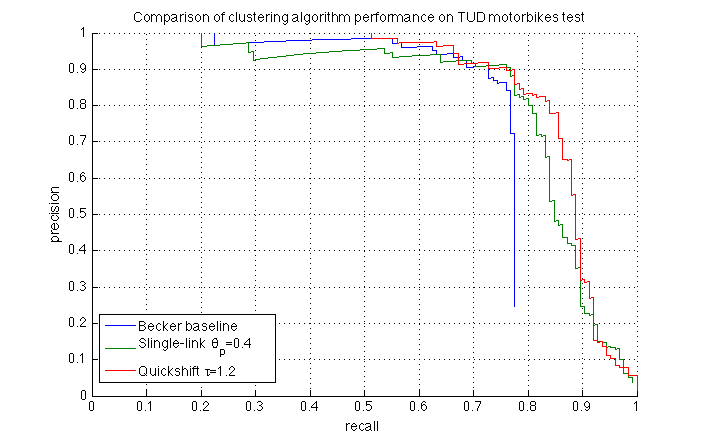
\includegraphics[width=0.8\textwidth]{TUD_k1_clusteralgs}
    \label{fig:tudk1clusteralgos}
    \caption{Precision-Recall curves of the TUD Motorbikes detection task, using Becker's \cite{becker2012codebook} setup as baseline, Single-link clustering with a maximal detection overlap of 0.4 and quickshift clustering with $\tau = 1.2$.}
\end{figure}

\begin{table}
    \begin{tabular}{rc|cc>{\bfseries}c}
        ~&k&no. of detections&total recall&average precision \\
        baseline&1&---&---&0.83 \\
        Becker's settings&1&394&0.7760&0.7536\\
        single-link $\theta_p=0.4$&1&3447&0.9920&0.8342\\
        quickshift $\tau=1.2$&1&7968&1.0000&0.8680\\
        quickshift $\tau=1.2$&4&8147&0.9680&0.8940
    \end{tabular}
    \label{tab:tudk1clusteralgos}
    \caption{Comparison of test statistics of TUD Motorbikes tests using various clustering algorithms and settings. \emph{Baseline} represents the result reported by Becker \cite{becker2012codebook}.}
\end{table}

Table \ref{tab:tudk1clusteralgos} shows some more statistics of the experiments. The results reported by Becker are somewhat higher than my own replication. This might be caused by a fortunate set of random background descriptors. Becker does not report the randomization process involved, so I was not able to replicate the results exactly. It also clearly shows that raising the $\theta_P$ threshold for the maximal overlap between detections should not be 0, because the recall gets much higher when it is set higher.


\todo[inline]{Results on VOC07?}

\begin{figure}[hbt]
    \centering
    \missingfigure[figwidth=0.8\textwidth]{Result graph VOC07}
\end{figure}


\begin{table}[hbt]
    \centering
    \missingfigure[figwidth=0.8\textwidth]{Result table VOC07}
\end{table}
% subsection exemplar_nbnn_results (end)

% section nbnn_detection (end)

\subsection{Exemplar-$k$NBNN Detection} % (fold)
\label{sec:local_nbnn_detection}
A downside of the exemplar-NBNN method is the descriptor aliasing problem explained in Section \ref{sec:descriptor_aliasing}. This can be solved by taking the $k$ of $k$NN to be greater than 1. This means that the $k$ closest neighbors over all classes (the object class and the background class) are taken into account when constructing detection hypotheses. Within these $k$ nearest neighbors, the ones belonging to the object class that are closer than any neighbor in the background class, are transformed into detection hypotheses. This $k$NBNN approach was tested in the detection algorithm and compared to the previous setup.

\subsubsection{Local NBNN Detection} % (fold)
\label{ssub:local_nbnn_detection}

Another disadvantage of exemplar-NBNN detection is it returning many false positive detections for images not having any objects of the current object class. The reason for this is obvious, as all descriptors closer to the class than to the background will be regarded as hypotheses, and therefore images without any objects get reasonably well ranked detections. This problem gets larger as the data sets contains more object classes.

A solution for this is to not only compare the current object class with the background class, but to compare it with all other classes, to see what each descriptor in the test image looks most like. This results in a hypothesis selection step that chooses only descriptors that are closer to the current class than to any other.

This however would create another problem not present in the original approach. Some descriptors could be an indication for multiple classes, because certain parts of objects are quite similar. While the original exemplar-NBNN approach allows for this, regarding each class independently, this multi-class approach prevents this. Think of the similarity of a bicycle wheel with that of a motorbike or a car. To disregard all but one of these classes might cause very little evidence for most classes in an image, giving less stable detections. This reminds of Boiman's argument that much evidence is vital for the NBNN method, because the Naive Bayes assumption is only met towards infinity and there is no training phase to compensate for it.\cite{boiman2008defense}

At the same time, the goal to compare all classes simultaneously is similar to McCann's formulation of local NBNN's query.\cite{mccann2012local} (\emph{cf.} Section \ref{sec:local_nbnn}). Merging all class indexes into one, and taking into account not only the first NN per class, but the $k$ NN \emph{overall} prevents having too many false positive results, while keeping the possibility of a descriptor to be used for a hypothesis for multiple classes like in the original problem.

As a bonus, local NBNN for detection also incorporates a way to prevent the aliasing problem. Among the $k$ closest neighbors, there might be multiple ones from the same class. Instead of disregarding these neighbors like local NBNN does, they can be taken into account by creating hypotheses for all non-background nearest neighbors.

% subsubsection local_nbnn_detection (end)

\subsubsection{LNBNN Results} % (fold)
\label{ssub:lnbnn_results}
\todo[inline]{Results of kNBNN, localNBNN both TUD motorbike and VOC07}



\begin{figure}[hbt]
    \centering
    \missingfigure[figwidth=0.8\textwidth]{Result graph TUD Motorbike, with kNBNN, localNBNN}
\end{figure}

\begin{figure}[hbt]
    \centering
    \missingfigure[figwidth=0.8\textwidth]{Result graph VOC07, with kNBNN, localNBNN}
\end{figure}

\begin{table}[hbt]
    \centering
    \missingfigure[figwidth=0.8\textwidth]{Result table TUD Motorbikes, kNBNN/localNBNN}
\end{table}

\begin{table}[hbt]
    \centering
    \missingfigure[figwidth=0.8\textwidth]{Result table VOC07, kNBNN/localNBNN}
\end{table}

% subsubsection lnbnn_results (end)
% section local_nbnn_detection (end)
% chapter experimental_setup (end)

\section{Analysis of Results} % (fold)
\label{cha:analysis_of_results}

The experiments and their results show a number of things: the approach of exemplar-NBNN detection works not only on the TUD dataset, but also fairly well on the VOC2007 set. Furthermore, the substitution of of the agglomerative clustering algorithm with a mode finding algorithm seems to have a positive effect, just like taking a value of $k>1$ and using LNBNN. Nevertheless there is much variance within the results, and therefore it is necessary to give a deeper analysis of the results, to find out how they can be interpreted.

\subsection{The Datasets} % (fold)
\label{sec:the_dataset}

The differences between the datasets are striking. The TUD Motorbikes set has a single class, and the test set contains only positive images (i.e. images with at least one motorbike). The training set has a clear-cut segmentation, which improves the feature quality. The VOC07 dataset is much harder. Every class appears in only 5\% of the test images, excluding the \emph{person} class, which occurs in 40\% of the images. To put it another way, in the TUD Motorbike test the task is for every image to locate the motorbike object(s), while in de VOC2007 test the task is for every image and every class to assess the possibility of this class having an object in the image, and if yes, to locate it.

Of course, in practice these tasks are modeled in the same way. The detections within a single class are all compared to one another in terms of their value (cluster size), across all images, both class and non-class images (\emph{Cf.} the PASCAL VOC evaluation method \cite{pascal-voc-2007}.)

Another important aspect is that the TUD dataset tends to have motorbike objects that are large, centered in the image, and with little clipping and occlusion. Some of the classes of VOC2007 consist of objects that are generally small (\emph{bottle}), not in the focal point of the image (\emph{chair, pottedplant}), or often occluded by other objects (\emph{diningtable}).

This makes it obvious that the scores overall are higher on the TUD Motorbikes test than on the VOC2007 test. It raises the question however whether exemplar-NBNN might perform relatively better, or worse, on the TUD motorbikes test than on the VOC2007 set. It is difficult to compare this to other methods, because the TUD set is not regularly used in the literature. It is possible however to visualize what kinds of objects in both tests are hard to detect, and which ones are easy. This might give more insight in the mechanics of the algorithm.

\todo[inline]{Give highest scoring hits for both methods (TP), highest scoring misses (FP), lowest of both. Give relationship between object size and AP, just like VOC does}

% subsection the_dataset (end)

\subsection{Clustering Algorithms} % (fold)
\label{sub:anal_clustering_algorithms}

Overall, the suspicion seems to be correct that quickshift should perform better than agglomerative clustering because of the more natural way of selecting a cluster center, i.e. a detection out of a cluster of hypotheses. The results however depend a lot on class, and are not always very obvious.

To see whether the clustering of hypotheses is needed at all, for some tests a comparison was made between the performance of the ranked detections versus ranking the hpyotheses. As a ranking method, Becker's $Q_H$ measure was used (Equation~\ref{eq:qh}). Figure~\ref{fig:hyprank}

\begin{figure}{hbt}
    \centering
    \missingfigure{Duration graph}
    % \includegraphics[width=0.8\textwidth]{hyprank}
    \caption{Comparison of Average Precision using the clustered detections versus the hypotheses before clustering, on a test with \ldots}
    \label{fig:hyprank}
\end{figure}
\todo{Make a figure with this.}

The recall of the detections will usually be lower than the recall when using hypotheses, because the detections are more or less a subset of hypotheses. However, ranking the hypotheses appears to be much harder than ranking detections, resulting in a much lower AP. This shows the main benefit of clustering.

% subsection clustering_algorithms (end)

\subsection{The Influence of $k$} % (fold)
\label{sub:the_influence_of_k_}

The experiments show that performance increases when multiple neighbors are taken into account, confirming the theory of descriptor aliasing in Section \ref{sec:descriptor_aliasing}. There is however a quite narrow sweet spot: setting $k$ too high hurts performance and, to an even larger extend, efficiency. \todo{write a small section on this sweet spot, and how k in LNBNN might ideally be higher, albeit time constraints}.


% subsection the_influence_of_k_ (end)

\subsection{Time and Memory} % (fold)
\label{sub:time_and_memory_constraints}

Detection algorithms can be compared not only for their qualitative performance, but also in terms of complexity and efficiency. Exemplar-NBNN is quite heavy in both terms. Given $t$ training images, $s$ test images, $d$ descriptors per image, on average, $c$ classes, and $k$ nearest neighbors, this is the time complexity breakdown of the main stages of the pipeline:
\begin{enumerate}
    \item Extracting features from the training images, splitting them into the classes, adding them to their respective NN indexes and saving their exemplars: $\frac{td}{c} \log \frac{td}{c}$, using FLANN kd-trees for building NN indexes.
    \item Extracting features from the test images: $s\times d$
    \item Finding $k$ nearest neighbors from each class, for each descriptor of each test image: $d s c \log \frac{td}{c} $, using kd-trees.
    \item Performing detection. For each test image and each class, get its hypotheses, calculated their pairwise overlap, and cluster them: $s c x\big((d k)^2\big)$, factor $x>1$ depending on the clustering algorithm, but at least once for the pairwise overlap.
\end{enumerate}

\begin{figure}{hbt}
    \centering
    \missingfigure{Duration graph}
    % \includegraphics[width=0.8\textwidth]{duration}
    \caption{Duration of various tests.}
    \label{fig:duration}
\end{figure}

\todo[inline]{explain and indicate what's important. Say something on memory complexity. Add something about no of descriptors in dsampling, compared with hlp.}

% subsection time_and_memory_constraints (end)


% section analysis_of_results (end)

\chapter{Conclusion} % (fold)
\label{cha:conclusion}

Since the introduction of NBNN in 2008, much efforts have been made improving the method for image classification, and to a lesser extend, object detection. Other approaches have been developing too, while NBNN still has the attention of a number of researchers, it has not (yet?) become a major approach in object recognition. This thesis explores the possibilities of NBNN into the domain of object detection, and confirms the appealing traits of the method also stated by others: training is quick, the pipeline is relatively straightforward and intuitive, with a number of theoretical benefits.

This thesis extends NBNN while keeping these traits intact. In the training phase, the only extension is keeping track of exemplars, which can be calculated easily. The pipeline is still intuitive, forming bounding-box hypotheses from NN features, clustering the hypotheses into detections, and ranking these. Introducing quickshift, a sound way of defining detections from clusters of hypotheses is devised. The theoretical basis of Local NBNN, in asking the question ``What do the features look like?'' instead of iteratively asking ``Does this feature look like class A? Like class B? \ldots'' is also in line with the simplicity of the NBNN approach, and at the same time it is theoretically more sound to look at the local neighborhood of features, instead of doing this on a per-class basis.

The resulting method improves over earlier NBNN-like methods for detection, and is capable of achieving good results on the popular benchmark image set of Pascal VOC 2007.

Having said this, the main disadvantage of this method, and earlier NBNN-based methods, is the slow test phase. Because no model is being learned, test images have to be compared with more or less raw training features, which is both complex in time and memory. Optimizations like FLANN relieve this complexity a bit, but the test phase remains a bottleneck. In detection, this disadvantage becomes even larger than in classification, because of the more extensive test phase. More research is needed to discover the practical boundaries of LNBNN detection and see what efficiency and performance improvements can be made.\\


% \section{Future Work} % (fold)
% \label{sec:future_work}

The focus on further research should be on finding efficient ways of performing object detection using NBNN. There might be ways of improving the clustering algorithm without hurting performance. For example, it would improve efficiency greatly if not every hypothesis would have to be compared to every single other one, by exploiting certain structural properties of bounding boxes.

It could also be interesting to try and combine the advantages of the NBNN approach with those of other detection methods, such as part-based models, efficient sub-window search, or hierarchical approaches. The object-to-class nature of NBNN might be a useful addition to these methods, that are often based on object-to-object distance measures. On the other hand, LNBNN detection might benefit from a more discriminative approach, such as support vector machines or conditional random fields.


% section future_work (end)

% chapter conclusion (end)
% \section{Discussion} % (fold)
\label{cha:discussion}
\todo[inline]{IDEA: perhaps as subsection, or integrated with Conclusion? Perhaps put it before Conclusion and see conclusion more as a small wrap-up? Or first wrap-up, then elaborate the causes? Give future work etc.}

\subsection{Future Work} % (fold)
\label{sec:future_work}

\todo[inline]{Talk about ...}
% section future_work (end)

% chapter discussion (end)

\bibliographystyle{is-plain}
\bibliography{ref}

\end{document}
